\chapter{Analysis}

\section{Introduction}

\subsection{Client Identification}

My client is Chranj Dingri; he is 50 years old and works for Volac int. as their IT Systems Manager. Volac int. is a company that produces and markets proteins, on a daily basis the company use computers in order to update and manage databases. Chranj's job includes building servers and installing operating systems on them, he also troubleshoots colleague's requests. In doing this job it means he has a lot of experience with computers and will be able to administrate the proposed system.


Chranj helps to allocate hardware devices to all co-workers in the business, it is very hard to keep track of who has what device and all the details that are linked with that device (warranties, amount paid for the device, make and model etc.). The hardware devices that he wants to keep track of are mobile phones, tablets, laptops, PCs and printers. With the new system Chranj would like to keep all his colleagues in a database and have it show which people have which device assigned to them, he would also like to see all the details about a specific hardware device. He would like the new system to be read only for colleagues looking at their own data and have only certain people being able to add entries and update information. Having this computer based system means that Chranj can have all the data he wants stored in one place so he can simply search for a colleague and get an overview of the devices assigned to them. 

\subsection{Define the current system}

Currently the system used is a spreadsheet on Excel. A customer will fill out a form manually on paper including their name and hardware devices they require, they then give it to their manager who will add an entry on the spreadsheet.  The spreadsheet stores the names of staff as well as which hardware device they have been allocated.

\subsection{Describe the problems}

A spreadsheet in Excel makes it easy to enter and read information however there are quite a few downsides to the current way of doing things. The first being that only a single user can edit the spreadsheet at a time, this means that if multiple people need to use the spreadsheet things start to get complicated. Another downside to the current system is that it is not available online to be able to login from a computer that does not have the spreadsheet already. The spreadsheet also does not have restricted access for particular people, if someone wants to view their hardware device information, they would also have full access to the spreadsheet which is not ideal as there is a security risk. With an Excel spreadsheet it is not very easy to search for a particular field (for example if someone wanted to search for a specific mobile phone) especially if there is a lot of data.

\subsection{Section appendix}

\begin{figure}[H]
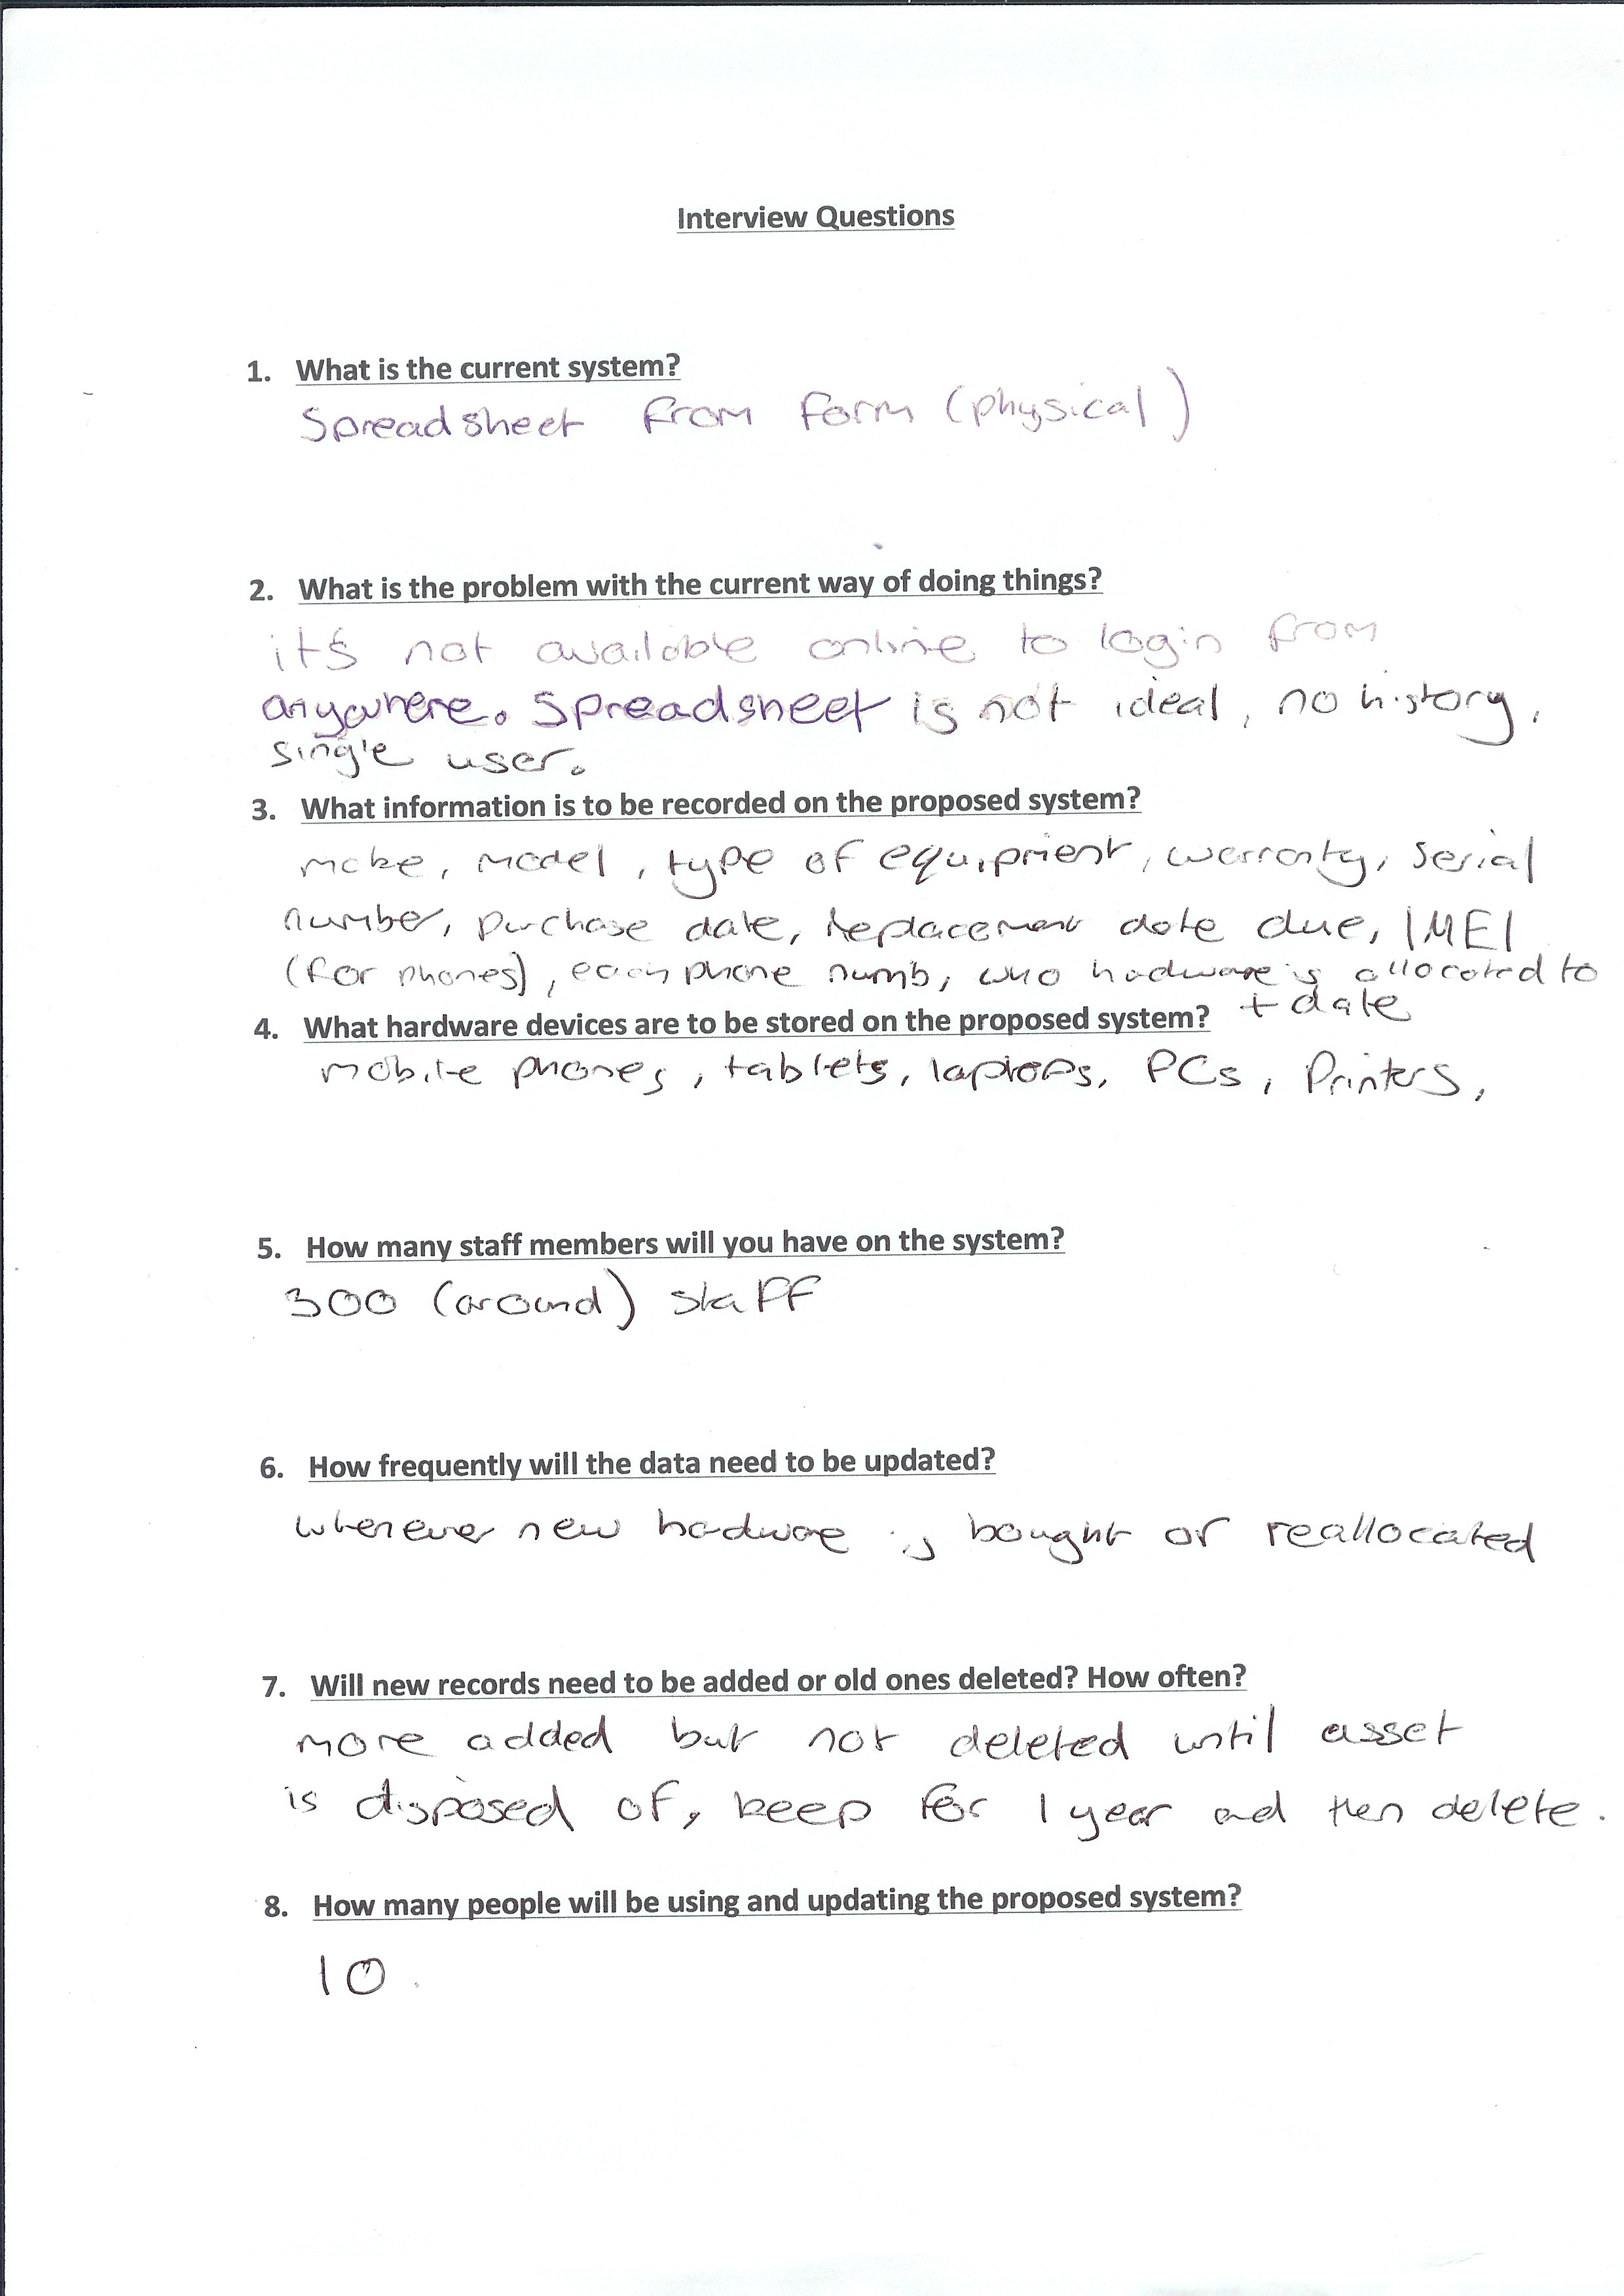
\includegraphics[width=.9\textwidth,height=.9\textheight,keepaspectratio]{Page1Interview.jpg}
\caption{Interview Questions: Page 2} \label{Page1Interview}
\end{figure}

\begin{figure}[H]
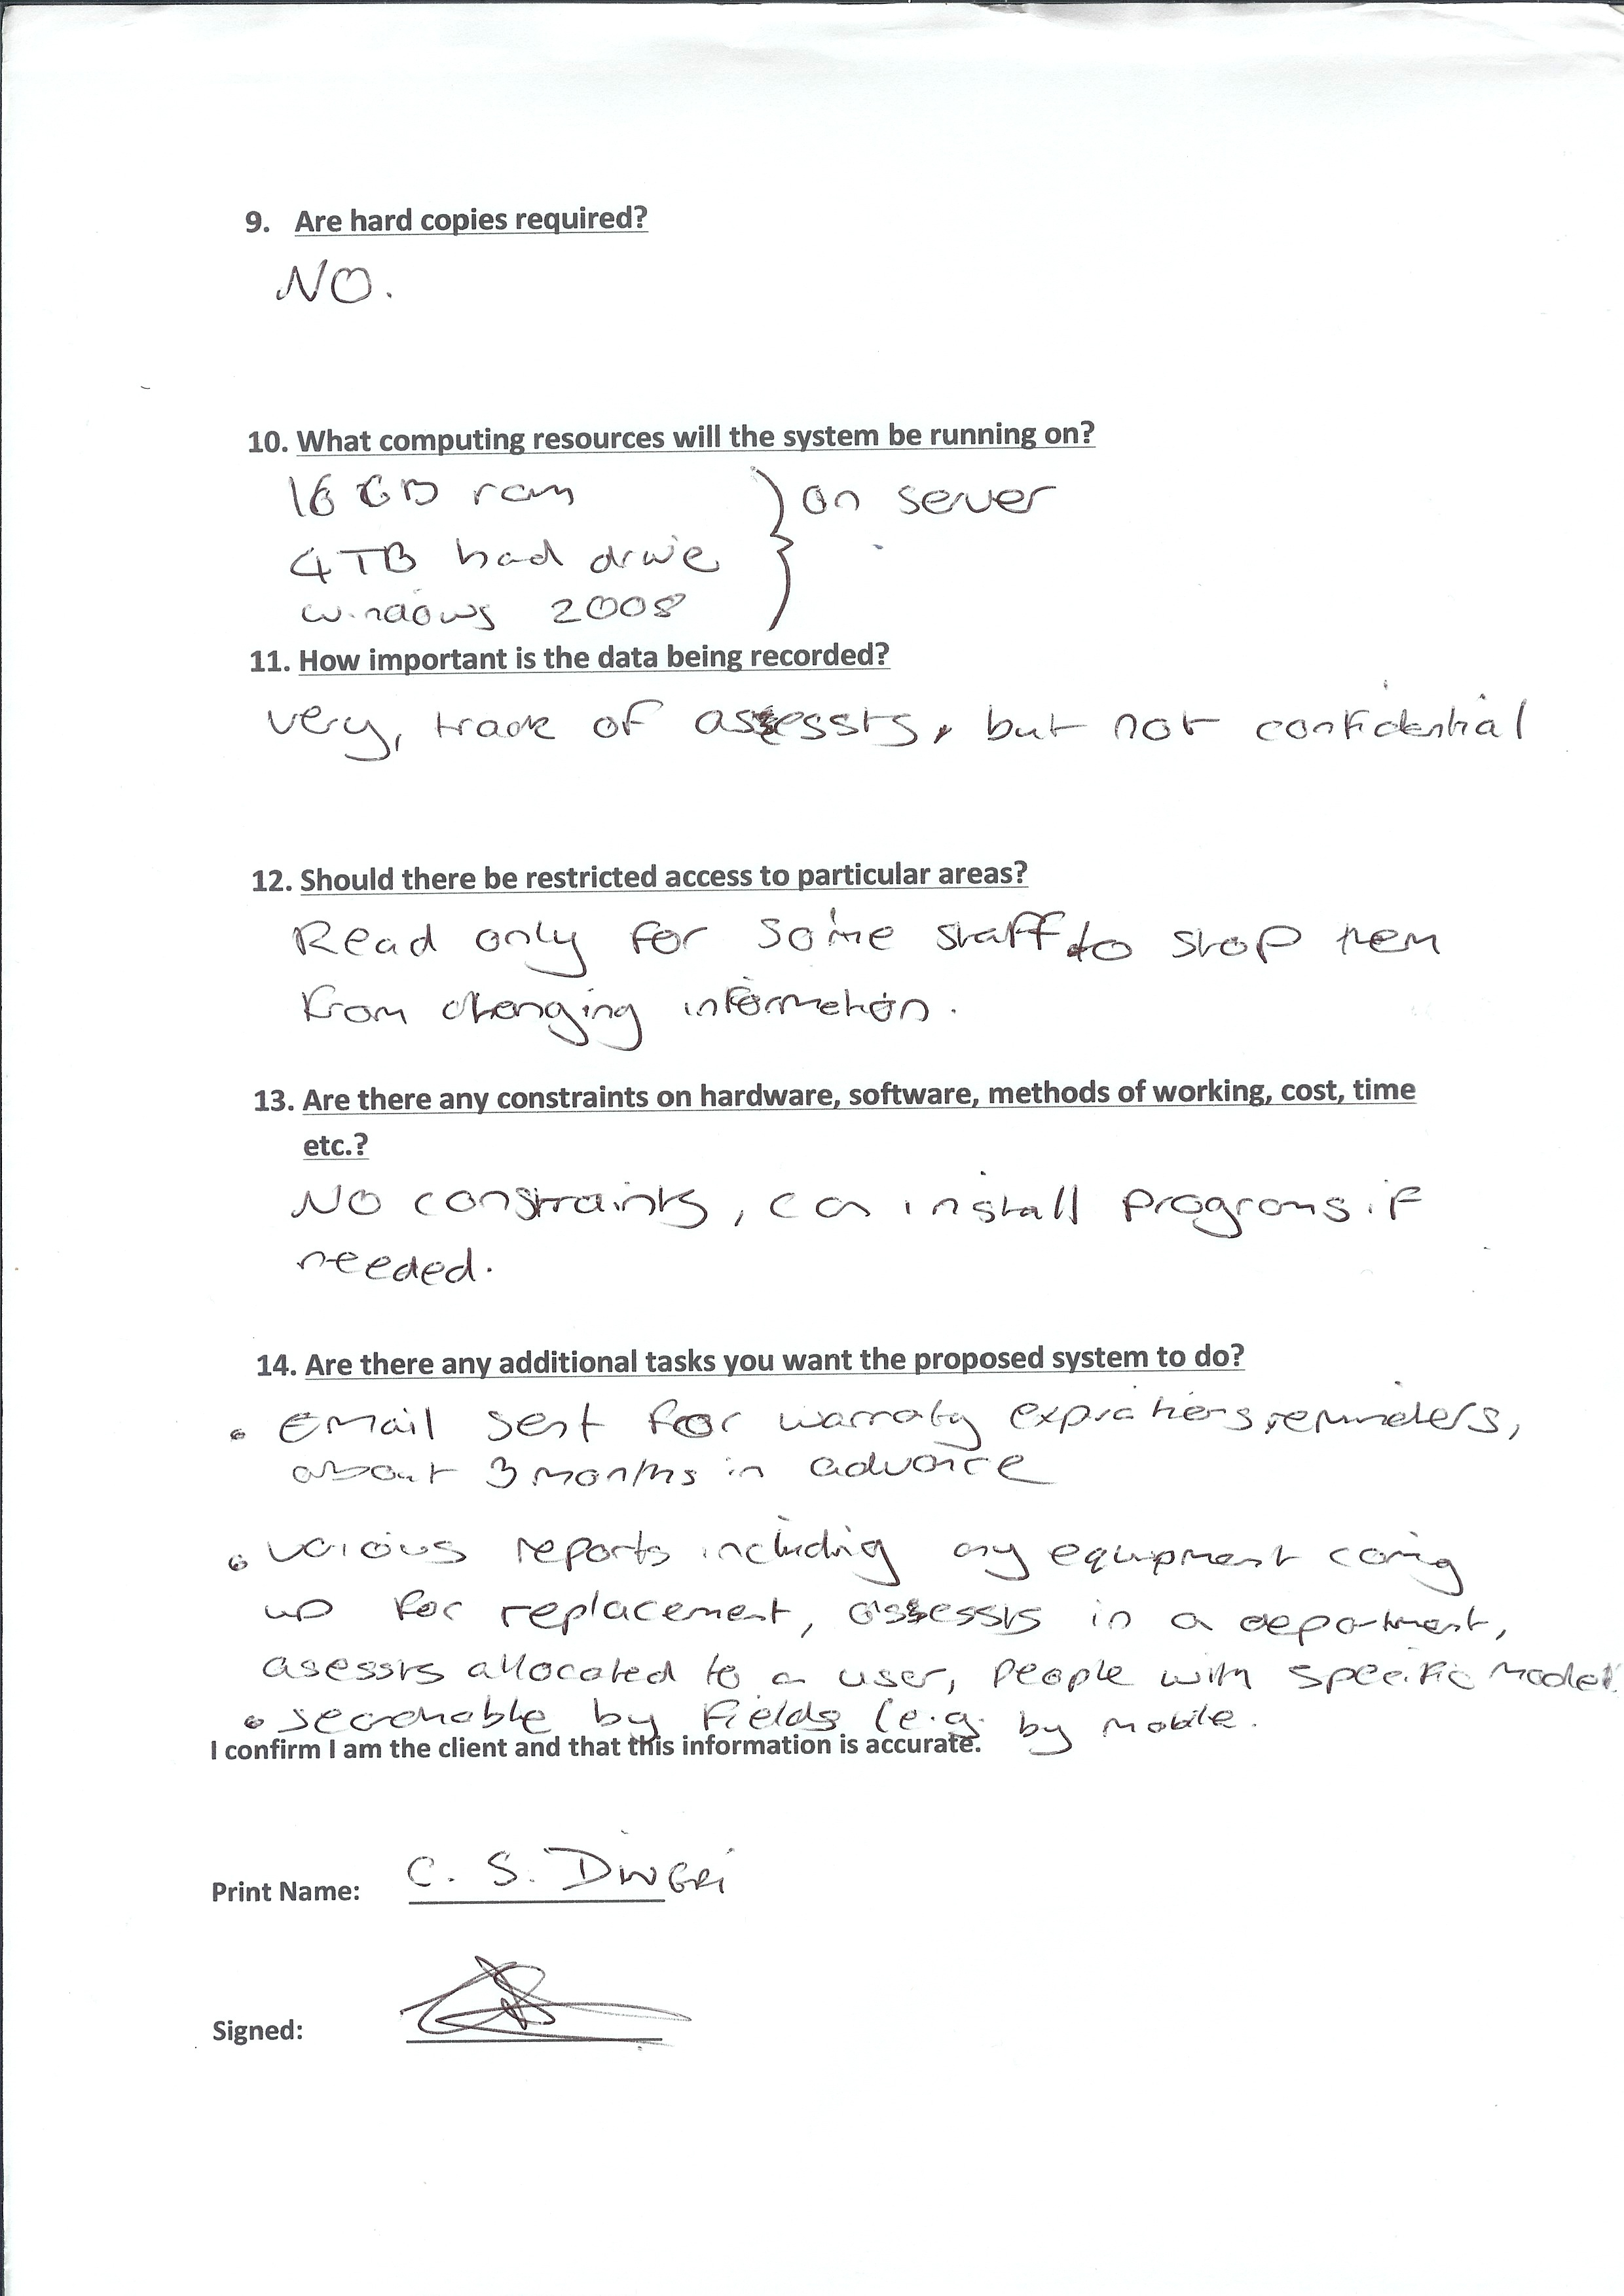
\includegraphics[width=.9\textwidth,height=.9\textheight,keepaspectratio]{Page2Interview.jpg}
\caption{Interview Questions: Page 2} \label{Page1Interview}
\end{figure}

\section{Investigation}

\subsection{The current system}

\subsubsection{Data sources and destinations}

In the current system there are three data sources used, the colleague, the line manager and the IT staff. Colleagues will fill out a physical form with information about which hardware device they would like to be assigned to them along with their name. The form will then be given to their specific line manager who will sign the form to say whether they authorize the hardware request or not. The line manager will give this form to a member of the IT staff who will enter the data onto the Excel spreadsheet along with the hardware details (such as cost and serial number). The spreadsheet now contains all the information about which colleague has which hardware device assigned to them.

\begin{table}[H]
\scalebox{0.65}{
\begin{tabular}{|p{4cm}|p{5.3cm}|p{8cm}|p{3cm}|}
\hline
\multicolumn{1}{|c|}{\textbf{Source}} & \multicolumn{1}{c|}{\textbf{Data}} & \multicolumn{1}{c|}{\textbf{Example Data}}         & \multicolumn{1}{c|}{\textbf{Destination}} \\ \hline
Colleague                             & First Name                         & John                                               & Form                                      \\ \hline
Colleague                             & Last Name                          & Smith                                              & Form                                      \\ \hline
Colleague                             & Department                              & Financing                                            & Form                                      \\ \hline
Colleague                             & Location                              & Orwell                                            & Form                                      \\ \hline
Colleague                             & Hardware Device Wanted             & Phone                                              & Form                                      \\ \hline
Colleague                             & Make                               & iPhone                                             & Form                                      \\ \hline
Form                                  & Form Details                       & John, Smith, Phone, iPhone                 & Line Manager                              \\ \hline
Line Manager                          & Signature                          & Tim Richardson                                     & Form                                      \\ \hline
Form                                  & Form Details Including Signature   & John, Smith, Phone, iPhone,Financing,Orwell, Tim Richardson & IT Staff Member                           \\ \hline
IT Staff Manager                      & Form Details Including Signature   & John, Smith, Phone, iPhone,Financing ,Orwell, Tim Richardson & Excel Spreadsheet                                   \\ \hline
IT Staff Member                             & Model                              & 6 Plus                                             & Excel Spreadsheet                                       \\ \hline
IT Staff Member                       & Cost                              & £400                                               & Excel Spreadsheet        \\ \hline
IT Staff Member                       & Serial Number                      & 71624                                          &  Excel Spreadsheet           \\ \hline
IT Staff Member                       & Purchase Date                      & 11/02/2015                                         &  Excel Spreadsheet           \\ \hline
\end{tabular}
}
\end{table}

\subsubsection{Algorithms}

\begin{algorithm}[H]
\begin{algorithmic}
\State $FormCompleted  \leftarrow False$
\If{$FormCompleted \leftarrow False$}
	\State Fill out form with all required fields
	\State $FormCompleted \leftarrow True$
\Else
	\State {Give to line manager}
\EndIf
\end{algorithmic}
\end{algorithm}

\begin{algorithm}[H]
\begin{algorithmic}
\State$Authorize \leftarrow False$
\While{$Authorize \leftarrow False$}
	\If{Line manager has a problem with hardware request}
		\State Discuss an alternative hardware device and update form
	\Else
		\State{$Authorize \leftarrow True$}
	\EndIf
\EndWhile
\end{algorithmic}
\end{algorithm}


\begin{algorithm}[H]
\begin{algorithmic}
\State $Entry_Added \leftarrow False$
\While{$Entry_Added \leftarrow False$}
	\State Check if hardware device is in stock
	\If {Hardware device is not in stock}
		\State Discuss the situation with line manager
	\Else
		\State Purchase hardware device
		\State Input hardware request form details
		\State Input receipt details including warranty, cost, serial and purchase date
		\State $Entry_Added \leftarrow True$
	\EndIf
\EndWhile
\end{algorithmic}
\end{algorithm}
		

\subsubsection{Data flow diagram}

\begin{figure}[H]
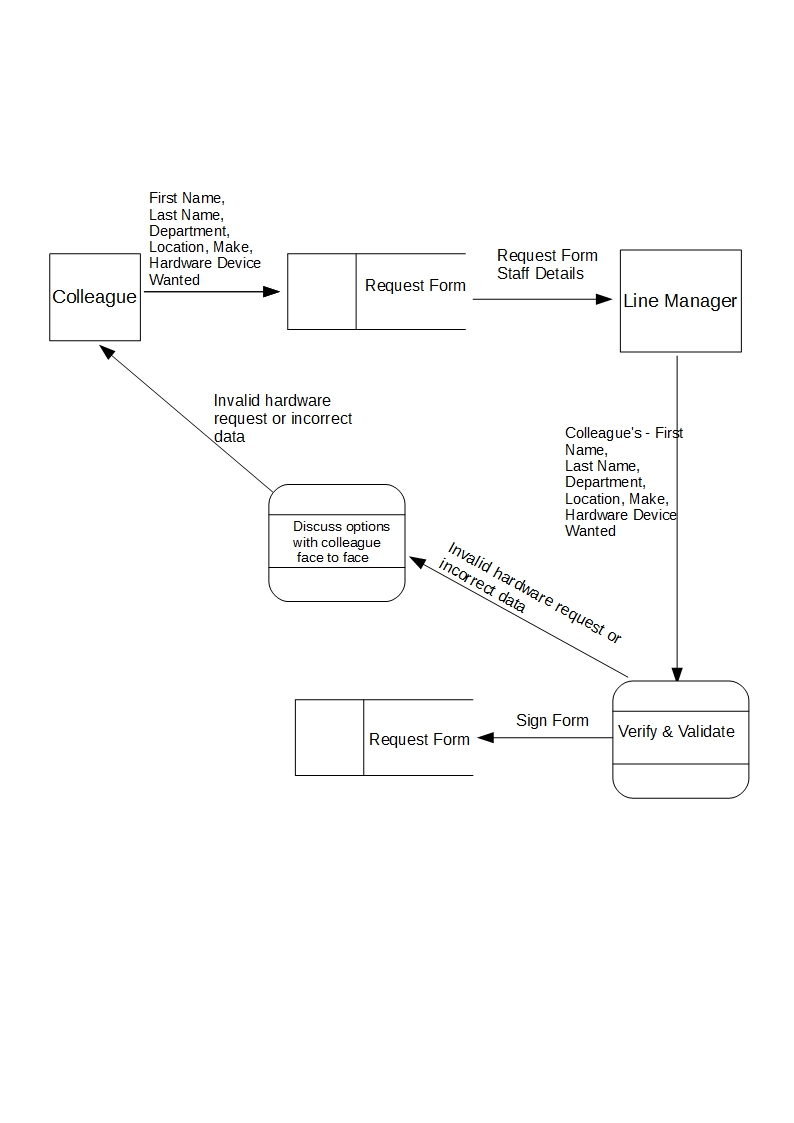
\includegraphics[width=\textwidth]{CurrentDFD.jpg}
\caption{A colleague filling in a hardware request form, this is then passed to the line manager for checking} \label{Page1Interview}
\end{figure}

\begin{figure}[H]
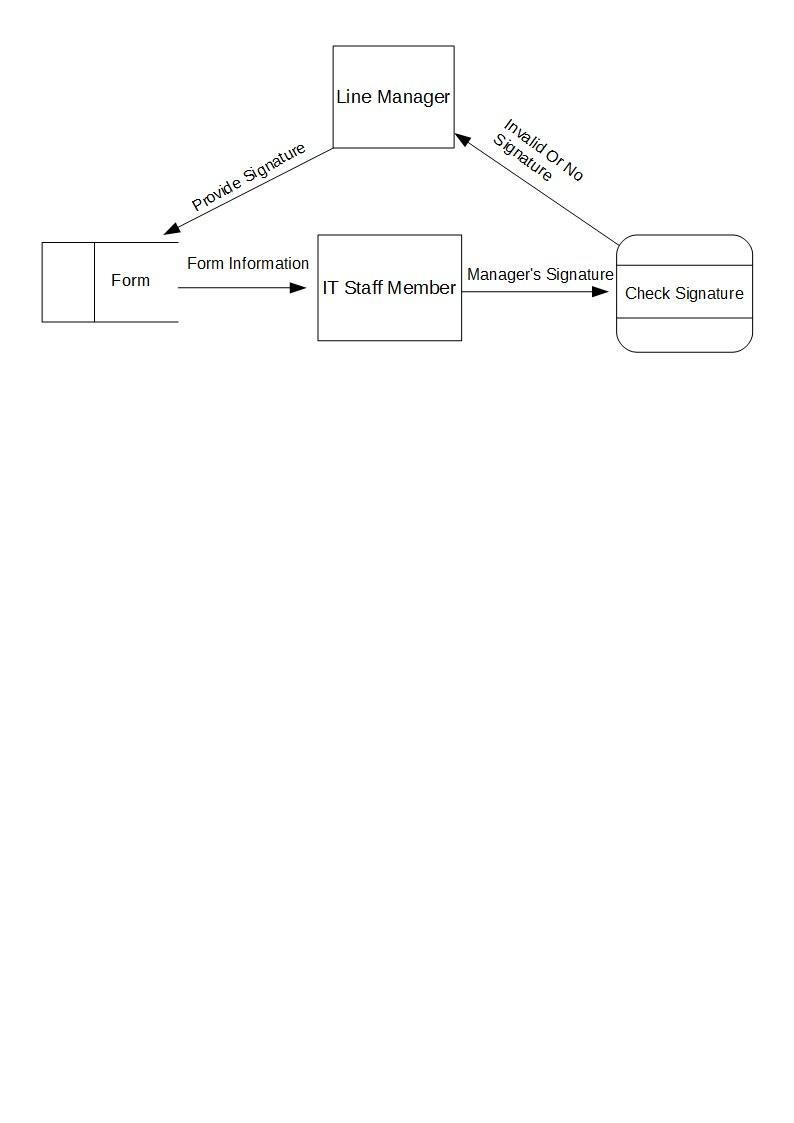
\includegraphics[width=\textwidth]{dataflowdiagram2.jpg}
\caption{The form is given to the IT staff who will check if the request form has a manager's signature } \label{Page1Interview}
\end{figure}

\begin{figure}[H]
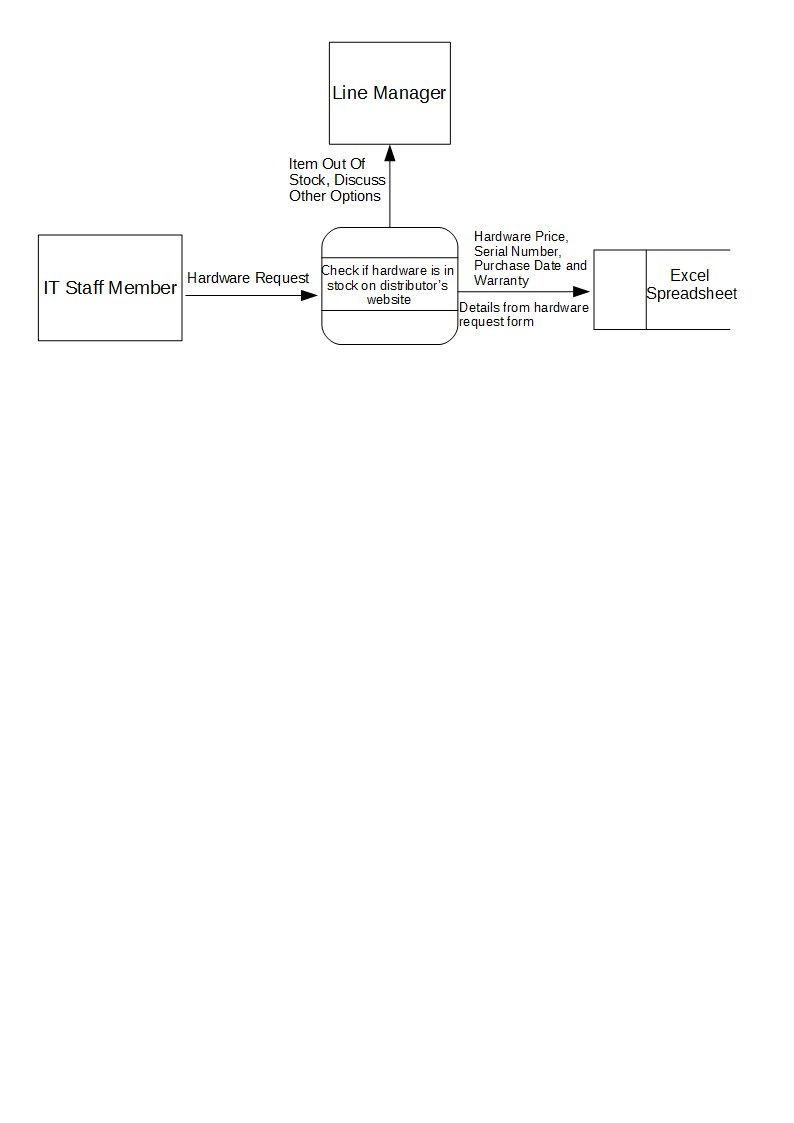
\includegraphics[width=\textwidth]{dataflowdiagram3.jpg}
\caption{The IT staff check with the company's distributer to check if the item is in stock, if it is not the manager is told. If the item is in stock, the information about the product is entered into the spreadsheet along with the details off the request form} \label{Page1Interview}
\end{figure}

\subsubsection{Input Forms, Output Forms, Report Formats}

\begin{figure}[H]
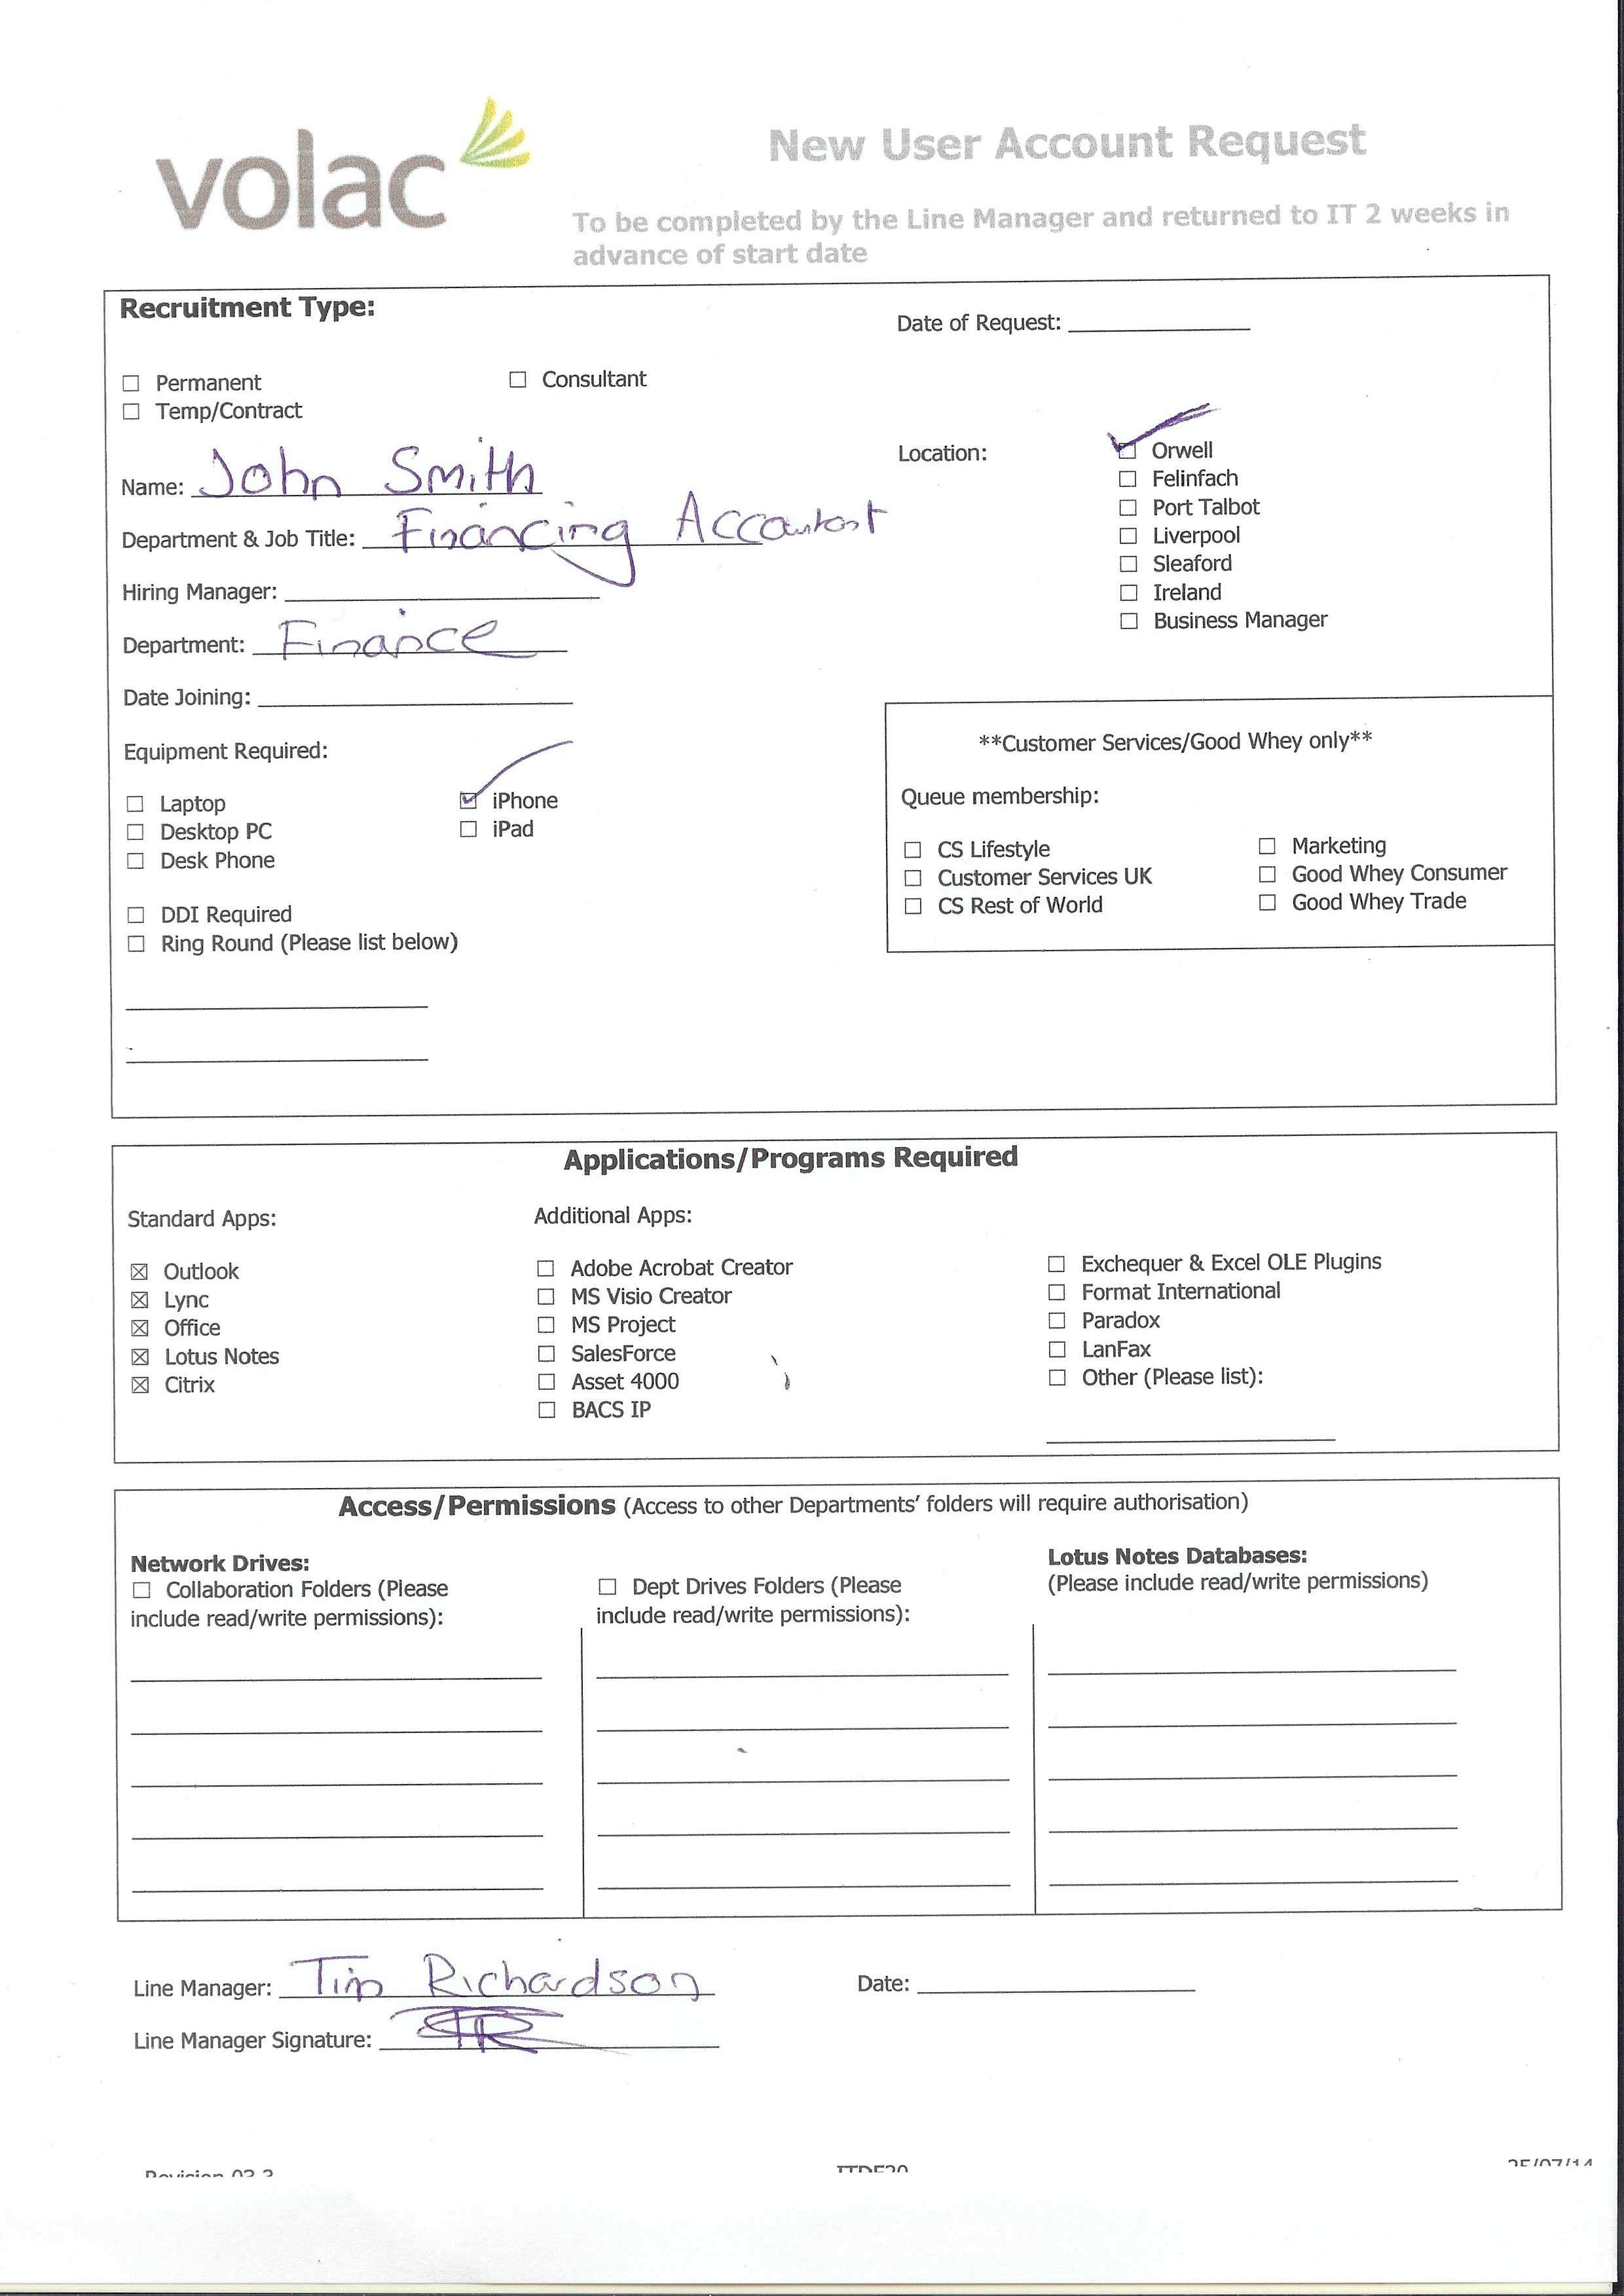
\includegraphics[width=.9\textwidth,height=.9\textheight,keepaspectratio]{HardwareRequestForm.jpg}
\caption{\textbf{The Hardware Request Form}:This document has only been filled in with the required details to be stored on the system. The rest of the details are not necessary to be stored in the hardware allocation system.} \label{HardwareRequestForm}
\end{figure}

\begin{figure}[H]
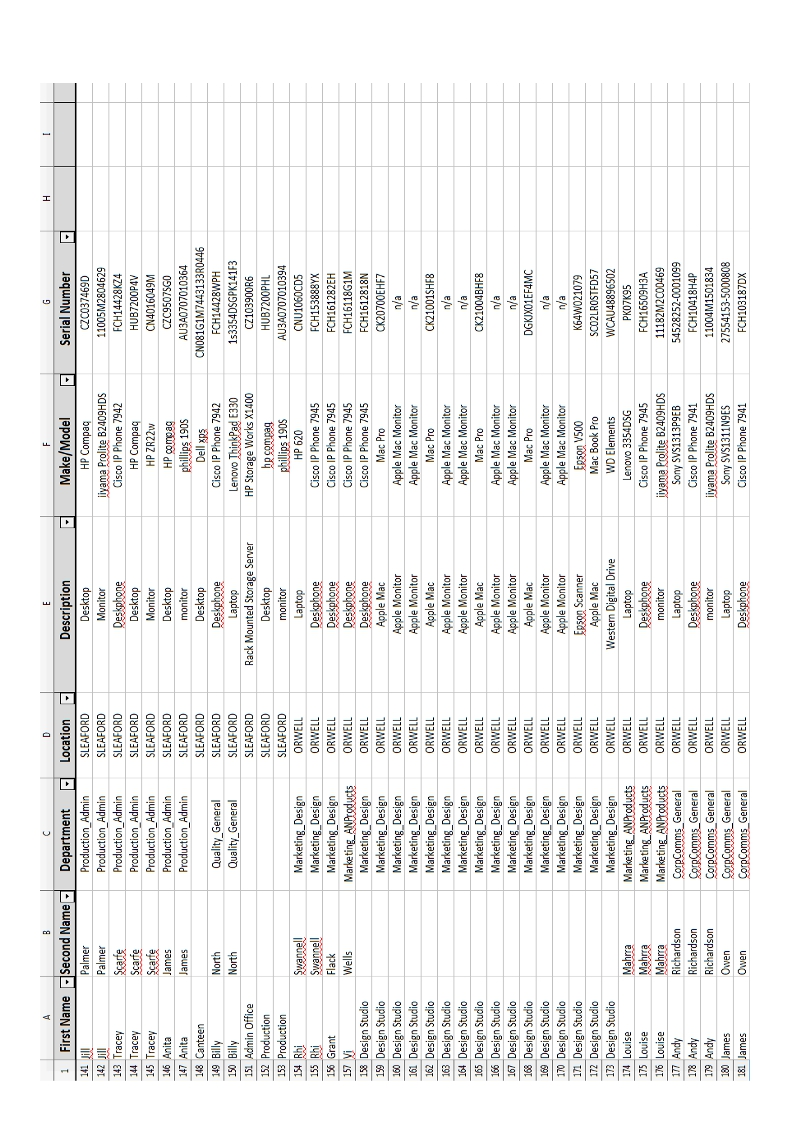
\includegraphics[width=.9\textwidth,height=.9\textheight,keepaspectratio]{Spreadsheet.jpg}
\caption{\textbf{The Hardware Allocation Spreadsheet}: As shown above the spreadsheet is not properly used by staff. Wrong data has been entered in the name box (see cell 172) and altogether the spreadsheet is messy. However it does store the necessary data for each person with their hardware devices.} \label{Spreadsheet}
\end{figure}


\subsection{The proposed system}

\subsubsection{Data sources and destinations}

In the proposed system collegue details and hardware requests will still be received via physical form and entered manually onto the system. The new system will store the same information from the colleagues however the IT staff will store more infomation on products such as IMEI numbers (for phones) (see question 3 in interview)

\begin{longtable}{|p{3cm}|p{3cm}|p{3cm}|p{3cm}|}
\hline
\multicolumn{1}{|c|}{\textbf{Source}} & \multicolumn{1}{c|}{\textbf{Data}} & \multicolumn{1}{c|}{\textbf{Example Data}}         & \multicolumn{1}{c|}{\textbf{Destination}} \\ \hline
Colleague                             & First Name                         & John                                               & Form                                      \\ \hline
Colleague                             & Last Name                          & Smith                                              & Form                                      \\ \hline
Colleague                             & Department                              & Financing                                            & Form                                      \\ \hline
Colleague                             & Job Title                              & Financing Manager                                          & Form                                      \\ \hline
Colleague                             & Location                              & Orwell                                            & Form                                      \\ \hline
Colleague                             & Make                              & iPhone                                             & Form                                      \\ \hline
Colleague                             & Hardware Device Wanted             & Phone                                              & Form                                      \\ \hline
Form                                  & Form Details                       & John, Smith, Phone, iPhone                & Line Manager                              \\ \hline
Line Manager                          & Signature                          & Tim Richardson                                     & Form                                      \\ \hline
Form                                  & Form Details Including Signature   & John, Smith, Phone, iPhone, Financing , Financing Manager, Orwell, Tim Richardson & IT Staff Member                           \\ \hline
IT Staff Manager                      & Form Details Including Signature   & John, Smith, Phone, iPhone, Financing , Financing Manager, Orwell, Tim Richardson & Database                                  \\ \hline
IT Staff Member                             & Model                              & 6 Plus                                             & Database (linked with colleague)                                      \\ \hline
IT Staff Member                       & Cost                              & £300                                               & Database (linked with colleague)          \\ \hline
IT Staff Member                       & Warranty                           & Yes                                        & Database (linked with colleague)          \\ \hline
IT Staff Member                       & Warranty Period                           & 3 Years                                            & Database (linked with colleague)          \\ \hline
IT Staff Member                       & Serial Number                      & 832327                                             & Database (linked with colleague)          \\ \hline
IT Staff Member                       & Purchase Date                      & 11/05/2015                                         & Database (linked with colleague)          \\ \hline
IT Staff Member                       & Phone Number (if phone)            & 07xxxxxxxxx                                        & Database (linked with colleague)          \\ \hline
IT Staff Member		&IMEI Number (if phone)            & EH37000781                                      & Database (linked with colleague)          \\ \hline	
\end{longtable}
\

\subsubsection{Data flow diagram}

\begin{figure}[H]
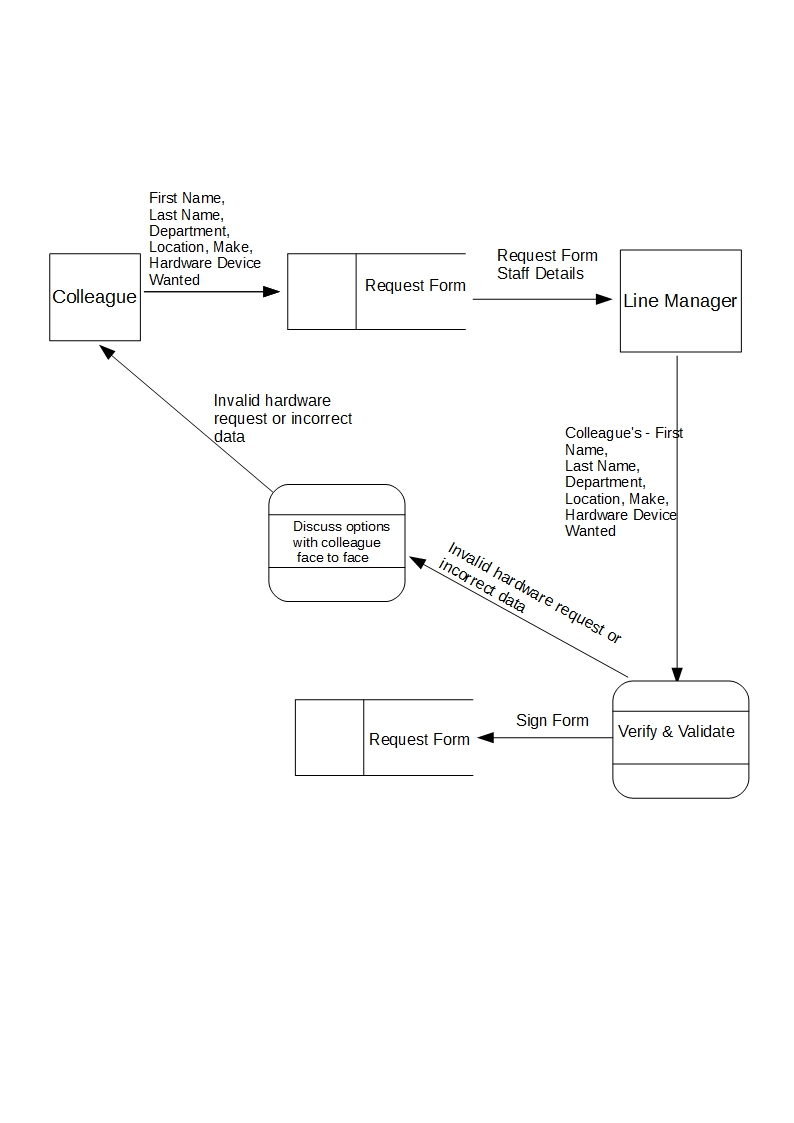
\includegraphics[width=\textwidth]{CurrentDFD.jpg}
\caption{This is the same process as with the last system. The colleague will fill in all necessary form details and give it to their line manager. The line manager will sign it and give it to the IT Staff.} \label{Page1Interview}
\end{figure}

\begin{figure}[H]
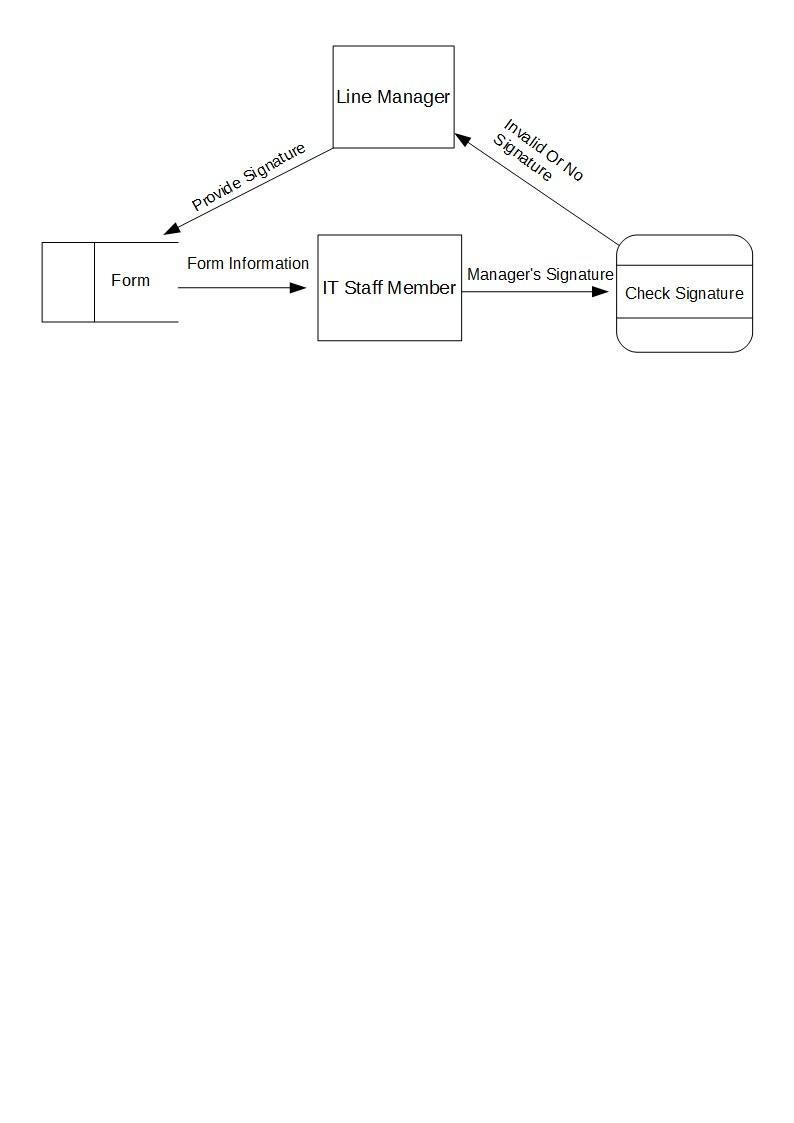
\includegraphics[width=\textwidth]{dataflowdiagram2.jpg}
\caption{This part of the system is also the same as the current system. The form is given to the IT staff who will check if the request form has a manager's signature } \label{Page1Interview}
\end{figure}

\begin{figure}[H]
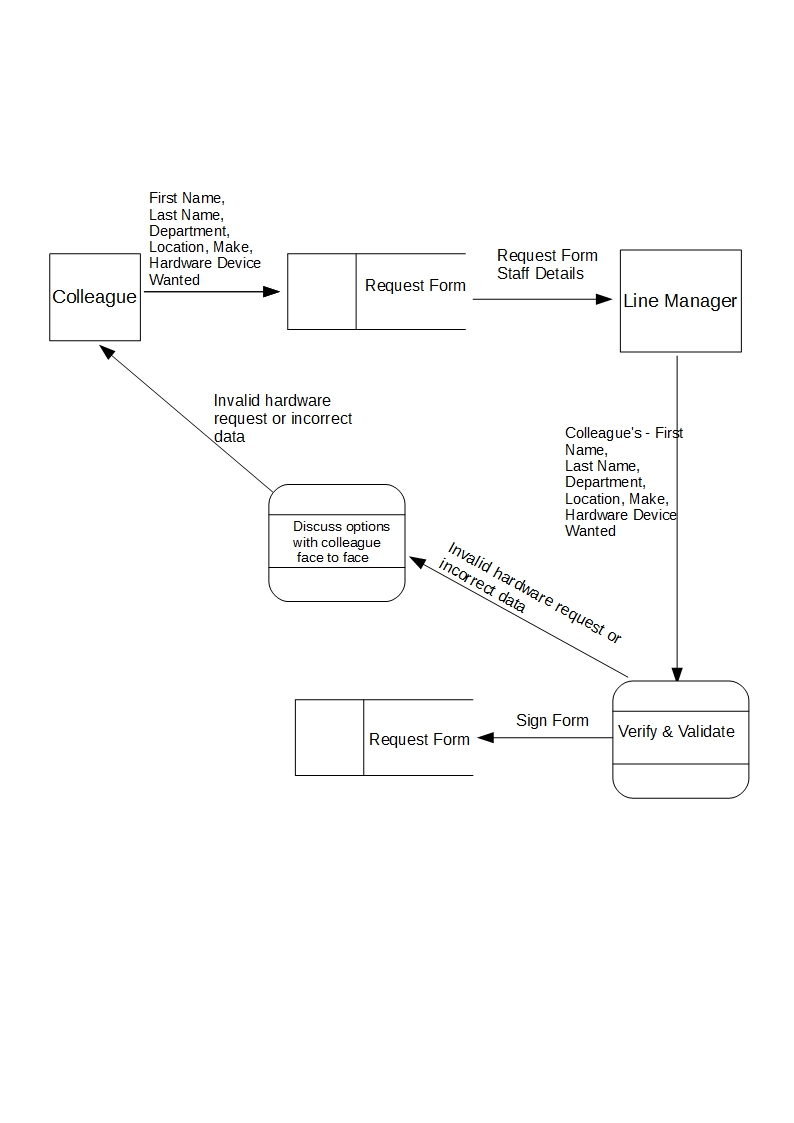
\includegraphics[width=\textwidth]{CurrentDFD.jpg}
\caption{This shows hardware information being entered onto the system. The IT Staff have their own login credentials to provide them with full access and they can then enter new data. After data has been added it will be necessary to log out again. } \label{Page1Interview}
\end{figure}

\begin{figure}[H]
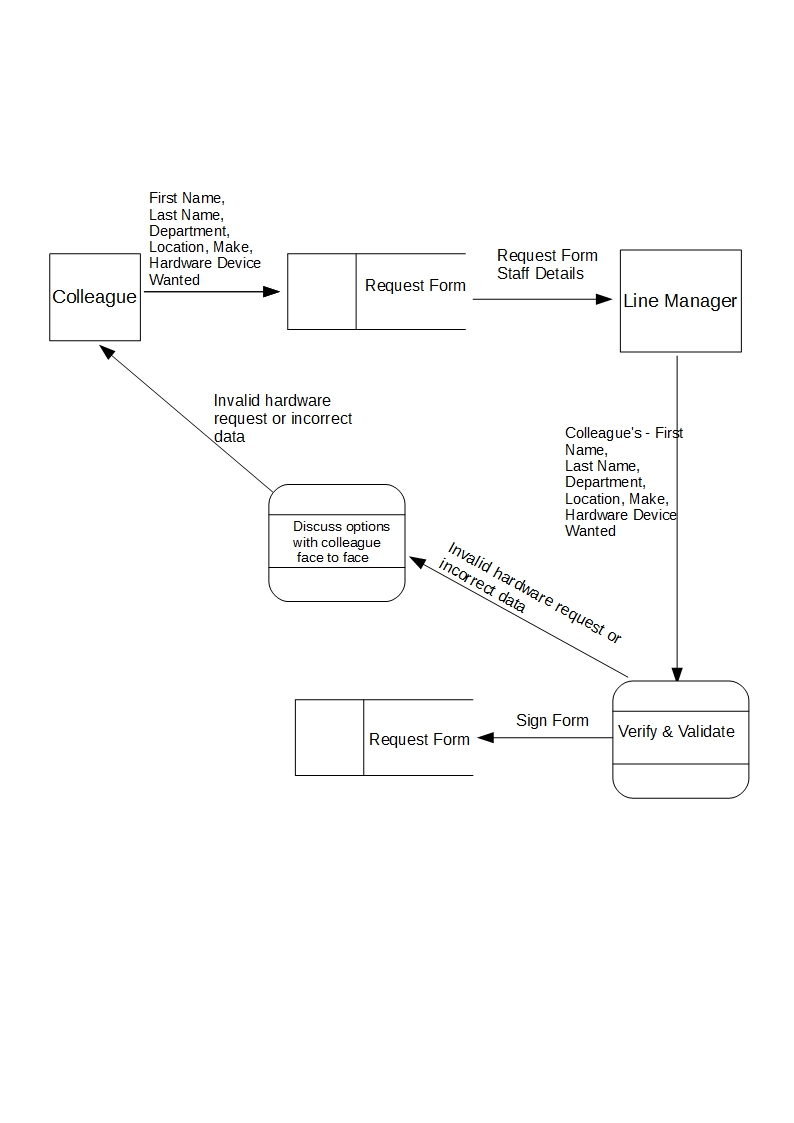
\includegraphics[width=\textwidth]{CurrentDFD.jpg}
\caption{This shows a colleague logging into the system to read their own data with read-only access. } \label{Page1Interview}
\end{figure}

\begin{figure}[H]
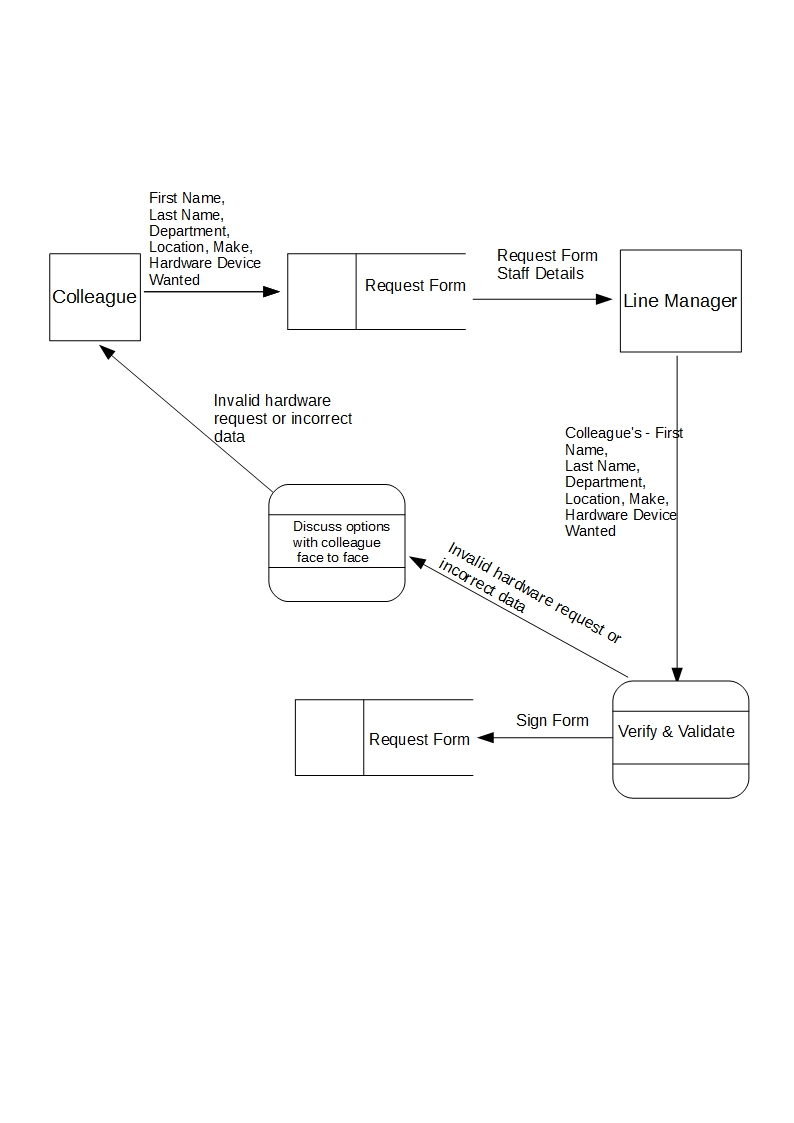
\includegraphics[width=\textwidth]{CurrentDFD.jpg}
\caption{This shows how managers also have read only access to check their own information just like their colleagues.} \label{Page1Interview}
\end{figure}

\subsubsection{Data dictionary}

\fontsize{8}{7}\selectfont

\begin{longtable}{|p{3cm}|p{1cm}|p{1cm}|p{3cm}|p{2cm}|p{3cm}|}
\hline
\multicolumn{1}{|c|}{\textbf{Name}} & \multicolumn{1}{c|}{\textbf{Data Type}} & \multicolumn{1}{c|}{\textbf{Length}} & \multicolumn{1}{c|}{\textbf{Validation}} & \textbf{Example Data} & \textbf{Comment}      \\ \hline
StaffID                             & Integer                                 & 1-200                                & Range                                    & 132                   & Unique to the staff   \\ \hline
StaffFirstName                      & String                                  & 1-25                                 & Presence Check                           & John                  &                       \\ \hline
StaffLastName                       & String                                  & 1-25                                 & Presence Check                           & Smith                 &                       \\ \hline
StaffDepartment                     & String                                  & 1-30                                 & Length                                   & Financing             &                       \\ \hline
StaffJobTitle			& String				& 1-30			& Length			& Finance Manager		&		\\ \hline
StaffLocation                       & String                                  & 1-20                                 & Length                                   & Orwell                &                       \\ \hline
HardwareID                          & Integer                                 & 1-200                                & Range                                    & 121                   & Unique to each device \\ \hline
HardwareDevice                      & String                                  & 1-25                                 & Length                                   & Phone                 &                       \\ \hline
HardwareMake                        & String                                  & 1-25                                 & Length                                   & iPhone                &                       \\ \hline
HardwareModel                       & String                                  & 1-25                                 & Length                                   & 5S                    &                       \\ \hline
HardwareCost                       & Integer                                 & 1-2000                               & Range                                    & £500                  &                       \\ \hline
HardwareWarranty                    & Boolean                                 &                                      & Presence Check                           & True                  &                       \\ \hline
HardwareWarrantyPeriod              & String                                  & 1-10                                 & Length                                   & 3 Years               &                       \\ \hline
HardwareSerialNumber                & String                                  & 1-50                                 & Length                                   & 12307321              &                       \\ \hline
HardwarePurchaseDate                & Date                                  &                                  & Format                                   & 11/03/2015              &                       \\ \hline
HardwareIMEI                & String                                  &          1-50                        & Length                                   & EH37000781               & Only required for phones                      \\ \hline
HardwarePhoneNumber                & String                                  &1-11                                  & Length                                   & 07927551125              &   Only required for phones                      \\ \hline
\end{longtable}
\normalsize
\subsubsection{Volumetrics}

Initially my system will store 350 different client records, I chose this amount because Chranj said he has around 300 staff in his company he has to store as soon as the system is available (Interview question 5). Since he said "around 300" it shows he is fairly unsure exactly how many, so 350 means that the system will provide room for anymore staff that were not counted in the interview. The company does not hire people everyday and since this database will only be storing staff members, 350 records gives a fair bit of room to enable Chranj (and other IT staff members) to get used to the system.

If each colleague on the new proposed system has 11 fields of data stored about them (see Data Sources and Destination table) and each field took up 1KB of storage space, that would mean to store 350 client records (the initial amount) the minimum storage space required would be:

1KB x 11 fields = 11Kb (per person)\\
11Kb x 350 = 3850Kb\\
3850Kb/8 = 3.85 MB\\

The system itself may then add on a few MB. So I would say a minimum of 8.85MB will be required to use the system.


\section{Objectives}

\subsection{General Objectives}

\begin{itemize}
\item An organised database to replace the current spreadsheet
\item A clear and easy to use database for IT staff to enter colleague data
\item  A clear and easy to understand layout for colleagues to see their hardware allocations
\end{itemize}

\subsection{Specific Objectives}

\begin{itemize}
\item Link colleagues to hardware devices (and their details)
\item An easy to use search function to find a specific field
\item Read-Only access for colleagues viewing their own information (with a log-in system to allow this)
\item  An automatic email sent to IT staff members reminding them that a warranty is running out
\item Sort data into catergories such as by departement
\end{itemize}

\subsection{Core Objectives}
\begin{itemize}
\item Login access - Restricted access for colleagues
\item Automated email reminders for warranty
\end{itemize}

\subsection{Other Objectives}

\begin{itemize}
\item Online method of sending hardware request forms to eliminate the need for physical copies
\item Online database to login from anywhere
\end{itemize}

\section{ER Diagrams and Descriptions}

\subsection{ER Diagram}

\begin{figure}[H]
\hspace*{-2cm}
\vspace*{5cm}
\setlength{\abovecaptionskip}{-320pt plus 3pt minus 2pt}
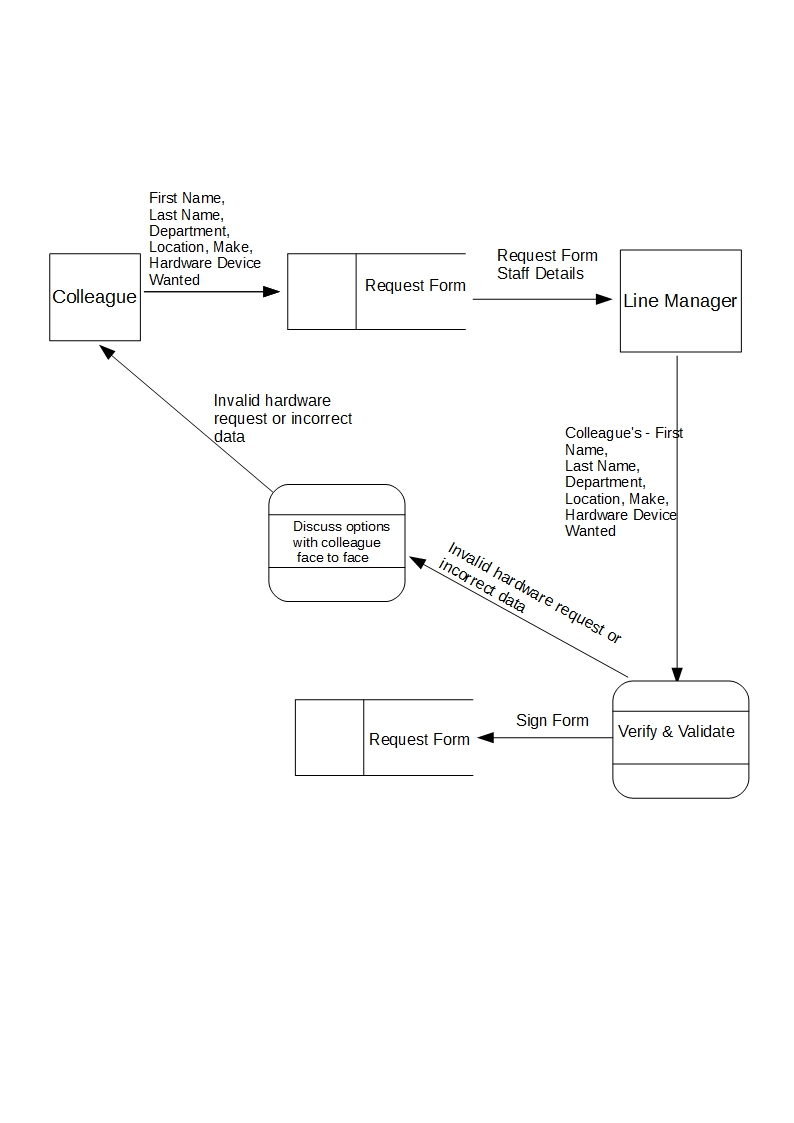
\includegraphics[width=1.2\textwidth]{CurrentDFD.jpg}
\caption{The ER Diagram is basic. Since the IT Staff and Line Managers also need their own hardware devices they are classified under the Staff table. All staff have many to many relationships with hardware as they can have a number of phones, printers, monitors etc. at one time.} \label{ER Diagram}
\end{figure}

\subsection{Entity Descriptions}

Staff(\underline{StaffID},\textit{HardwareID}, FirstName, LastName, Department, Location)

Hardware(\underline{HardwareID}, HardwareDevice, Make, Model, Cost, Warranty, \\WarrantyPeriod, SerialNumber, PurchaseDate)

\section{Object Analysis}

\subsection{Object Listing}

\begin{itemize}
\item Colleagues
\item Hardware
\item Line Mangager
\item IT Staff
\end{itemize}

\subsection{Relationship diagrams}

\begin{figure}[H]
\hspace*{-1.3cm}
\vspace*{-1cm}
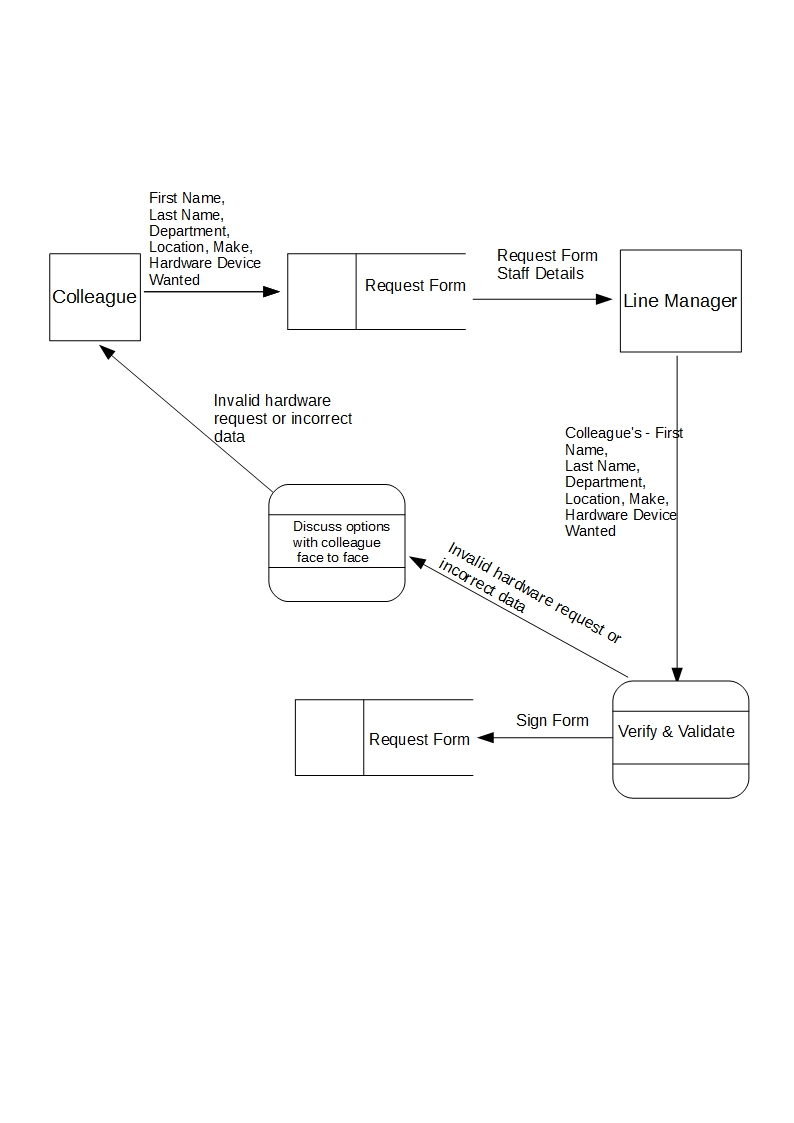
\includegraphics[width=1\textwidth]{CurrentDFD.jpg}
\caption{The class definitions show all the attributes for the class staff and the class Hardware. All staff (no matter if they are a manager or IT staff) will enter their data the same. Under the line shows all the methods for this class. Which currently are all edit and add methods.} \label{Relationship Diagrams}
\end{figure}

\subsection{Class definitions}

\begin{figure}[H]
\hspace*{-1.3cm}
\vspace*{-1cm}
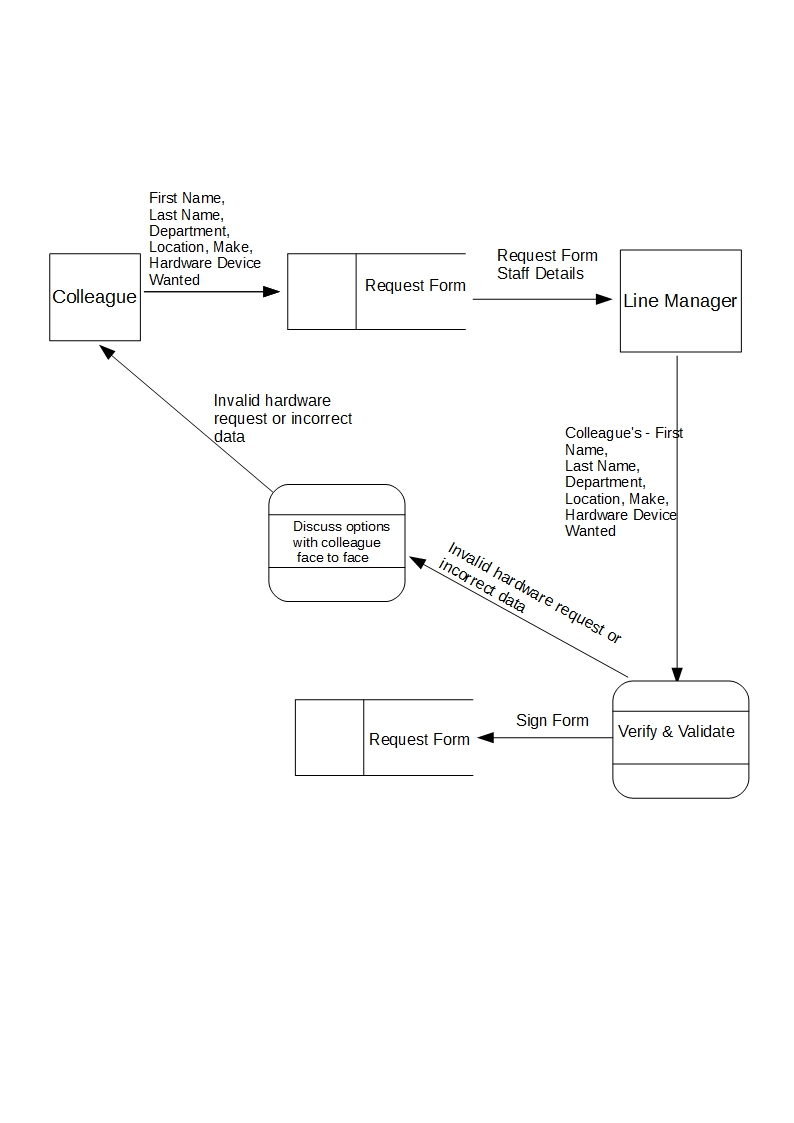
\includegraphics[width=1\textwidth]{CurrentDFD.jpg}
\caption{The relationship table shows the different staff related to my proposed system. They all get assigned hardware devices in the system and the IT staff will help all staff. The line managers are in charge of the colleagues in their department.} \label{Class Definitions}
\end{figure}

\section{Other Abstractions and Graphs}

\section{Constraints}

\subsection{Hardware}

The system will be stored onto a server stored in the workplace which is perfectly capable to handle the system, the specs are as followed:

\begin{itemize}
\item HP DL360
\item Windows 2003 (can run any operating system required)
\item 4TB Hard Drive
\item 16GB RAM
\item Quad Core Processor - 2.5 GHZ
\end{itemize}

The server is stored in a server room with high ventilation and fans operated 24/7. This is a huge benefit because the system can be running at all times so people can access the database.

\subsection{Software}

There is no real problem here, in the interview Chranj mentioned there are "no contraints" and I can install any programs if needed (question 13). There is a lot of hard disk space so the size of installations should not be a problem, the company runs on a fibre optic network with 100mb/s download speed so any downloads should be completed quickly.

\subsection{Time}

The only deadline is that given by the teacher on the 17th April 2015. However Chranj has said that "the earlier, the better" and will be happy to start using the system if it is finished early.

\subsection{User Knowledge}

Chranj works as an IT systems manager (see client identification) so he is perfectly qualified to deal with generic IT problems. However he has never used SQL and database software on a professional level so it will be necessary to provide him with a user manual to help with the software and to deal with any problems.

\subsection{Access restrictions}

One of the objectives for this program is to provide IT staff with full access rights to add/delete entries, and read-only rights to colleagues wanting to view their current hardware allocations and details. The program will be made like this because it reduces any security issues and means that if a certain colleague was given a better piece of hardware (such as a iPhone) other colleagues will not know and conflicts can be avoided.

\section{Limitations}

\subsection{Areas which will not be included in computerisation}

The physical form that colleagues will fill in to say which hardware device they would like, which the line manager then signs, will stay the same. This is because I feel signing a paper document is easier than signing on a computer, also I do not think a computerised version of this would make things any easier.

\subsection{Areas considered for future computerisation}

The hardware request forms may be computerised if there is enough time, the benefit this brings is that a computerised form is harder to misplace than a physical form. There will still need to be a way of allowing managers to sign off forms, this would be done by colleagues sending the form to managers, the managers providing an "Agree" or "Disagree" statement (by buttons instead of typing), and then forwarding the form to IT staff.

\section{Solutions}

\subsection{Alternative solutions}

\begin{center}
\begin{tabular}{|p{2.5cm}|p{3cm}|p{3cm}|p{3cm}|}
    \hline
    \textbf{Solution} & \textbf{Explanation} & \textbf{Advantages} & \textbf{Disadvanages} \\ \hline
Excel Spreadsheet & Improving and adding new fields to the existing excel spreadsheet. & \begin{itemize} \item Company already knows how to use it. \item Already on computer systems in workplace \end{itemize} & \begin{itemize} \item Linking data together is hard \item Data is unnecessarily repeated \end{itemize}  \\ \hline
Microsoft Access & Using Access to produce a database & \begin{itemize} \item Fairly easy to use as there is a user friendly GUI \item A great way to link tables/data together\end{itemize} &  \begin{itemize} \item Programming is not used \item The company has not been trained how to use it \end{itemize}  \\ \hline
Command-Line Application &		 Using a command line in python to provide a text display & 		\begin{itemize} \item Command line is very fast when handling data \item Easier to design \end{itemize} & 		\begin{itemize} \item Not user friendly as there is no GUI \item Hard to learn commands \item Not an upgrade from spreadsheet \end{itemize} \\ \hline
Web Based Application &		 Using online services  & 		\begin{itemize} \item Access from anywhere (meets client needs) \item Available to use by multiple people \item User friendly \end{itemize} & 		 \begin{itemize} \item Company will have to learn how to use it \item  Extra security needed (log-ins) \item Will be hard to program.\end{itemize} \\ \hline
PyQt GUI Application &		 Providing a GUI interface for the database using PyQt & 		\begin{itemize} \item GUI interface means it is easy to use for staff \item I will be learning PyQt in class to help with this solution \end{itemize} & 		 \begin{itemize} \item Cannot be logged on from anywhere \item Not ideal as it does not fully reach the 		     clients needs \end{itemize} \\
 \hline
\end{tabular}
\label{tab:range_examples}
\end{center}


\subsection{Justification of chosen solution}

The ideal solution is to use a web based application. However due to the fact it will take a long time to learn and implement this solution is placed in the "other objectives" section. The solution I will be using is a PyQt application, I will be using PyQt in class and already have a clear understanding of how to use it which will make implementation much faster. PyQt also provides a nice GUI for staff to use.